	\documentclass[aspectratio=169]{beamer}

\mode<presentation>
{
\usetheme{Darmstadt}%Darmstadt,Frankfurt

\setbeamercovered{transparent}
}
%Deutsche Silbentrennung
\usepackage[ngerman]{babel}
%Deutsche Umlaute
\usepackage[utf8]{inputenc}
%Listen einr�cken
\usepackage{enumitem}
% font definitions, try \usepackage{ae} instead of the following
% three lines if you don't like this look
\usepackage{mathptmx}
\usepackage[scaled=.90]{helvet}
\usepackage{courier}
%Trennung von deutschen Umlauten
\usepackage[T1]{fontenc}
\usepackage{adjustbox}
\usepackage{url}

\title{Projektarbeit: Háblame - das sprechende Faultier}

%\subtitle{}

% - Use the \inst{?} command only if the authors have different
%   affiliation.
%\author{F.~Author\inst{1} \and S.~Another\inst{2}}
\author{David Artmann\inst{1} \and Dominik Hirsch\inst{1} \and Kristoffer Schneider\inst{1}}

% - Use the \inst command only if there are several affiliations.
\institute[Universities of]
{
\inst{1}
Hochschule für angewandte Wissenschaften\\
Würzburg-Schweinfurt
}

\date{\today}


% This is only inserted into the PDF information catalog. Can be left
% out.
\subject{Talks}



% If you have a file called "university-logo-filename.xxx", where xxx
% is a graphic format that can be processed by latex or pdflatex,
% resp., then you can add a logo as follows:
\pgfdeclareimage[height=0.5cm]{university-logo}{media/logo/fhws.png}
\logo{\pgfuseimage{university-logo}}



% Delete this, if you do not want the table of contents to pop up at
% the beginning of each subsection:
\AtBeginSubsection[]
{
\begin{frame}<beamer>
\frametitle{Gliederung}
\tableofcontents[currentsection,currentsubsection]
\end{frame}
}

% If you wish to uncover everything in a step-wise fashion, uncomment
% the following command:
\beamerdefaultoverlayspecification{<+->}

\begin{document}
% titlepage
\begin{titlepage}
	%Eine mbox wird verwendet um Text zusammenzuhalten
	%vspace erzeugte die in Klammern angegebenen Zeilenabstände
	%baselineskip setzt zeilenabstand
   	\mbox{}\vspace{5\baselineskip}\\
   	%Schriftart und Größe als Attribut
   	\rmfamily\huge
   	%Mittige Textausrichtung (\centerline für eine Zeile)
   	\centering
   	%Das Argument erscheint in Kapitaelchen (small capitals).
	\textsc{Weiterentwicklung von Hablame}
	%Umbruch bezogen auf die Hoehe des Kleinbuchstaben x in diesem Element * Faktor
	\\[3ex]
   	Projektarbeit
   	\rmfamily\Large
   	\vspace{1\baselineskip}\\
   	%Externes einbinden einer Textdatei
   	%% versionsnummer entfernt
   	%\input{version.txt}\mbox{}
	\vspace{3\baselineskip}
	Hochschule für angewandte Wissenschaften Würzburg-Schweinfurt
   	\vspace{5\baselineskip}\\
   	\rmfamily\Large
   	David Artmann\\
   	\rmfamily\Large
   	Dominik Hirsch\\
   	\rmfamily\Large
   	Kristoffer Schneider
   	\vspace{1\baselineskip}\\
   	%Heutiges Datum
   	\today
\end{titlepage}
% toc
\begin{frame}
	\frametitle{Gliederung}
	\tableofcontents
	% You might wish to add the option [pausesections]
\end{frame}

\section{Projektziele}
	\begin{frame}
\begin{block}{}
	Strukturieren und Organisieren der Versionsverwaltung
\end{block}
\begin{block}{}
	Erstellen einer Dokumentation und eines Online-Nachschlagewerks
\end{block}
\begin{block}{}
	Stabilisieren und Erweitern des bisherigen Backends (Chatbot)
\end{block}
\begin{block}{}
	Einführung moderner Technologien und eines offenen DB-Systems
\end{block}
\begin{block}{}
	Realisieren einer Platform für Projektmanagement
\end{block}
\begin{block}{}
	Überarbeiten der Android App
\end{block}
\end{frame}		
\section{Organisatorisches}
	\subsection{Redmine}
		\begin{frame}
\begin{block}{}
	Dokumentation der Projektstruktur, API und Teilprojekte
\end{block}
\begin{block}{}
	Sammlung themenrelevanter und hilfreicher Links
\end{block}
\begin{block}{}
	Ticketsystem zur Veranschaulichung des Fortschritts und der Übersichtsschaffung
\end{block}
\begin{block}{}
	Groupware Fähigkeit (E-Mail, Kalender, News)
\end{block}
\end{frame}		
	\subsection{Versionsverwaltung (GitHub)}
		\begin{frame}
\center{\textbf{Alte Struktur}}
\begin{block}{}
	Alle Teilprojekte in einem Repository
\end{block}
\begin{block}{}
	Ein GitHub User von allen Projektteilnehmern genutzt
\end{block}
\begin{block}{}
	Altlasten vergangener Projekte
\end{block}
\begin{block}{}
	Fehlende Dokumentation
\end{block}
\begin{block}{}
	Verwendung schwacher Passwörter
\end{block}
\end{frame}
		\begin{frame}
\begin{block}{}
	Bisher: alle Teilprojekte in einem Repository auf GitHub
\end{block}
\begin{block}{}
	Jetzt: aufgeteilt auf einzelne Repositories
\end{block}
\begin{block}{}
	\begin{itemize}\itemsep0pt
		\item Háblame Android App (Java, Gradle, Android SDK)
		\item Háblame Service API Library (Java, Maven, Unirest)
		\item Háblame Botbackend (Java, Maven, Spring, AliceBot)
	\end{itemize}
\end{block}
\end{frame}
	\subsection{Dokumentation}
		\begin{frame}

\begin{block}{}
	Teil der Dokumentation im Redmine Wiki
\end{block}
\begin{block}{}
	Dokumentation des Codes mittels JavaDocs
\end{block}
\begin{block}{}
	Pro Repository ein Readme mit Basisinformationen
\end{block}
\end{frame}
\section{Teilprojekte}
	\subsection{Android App}
		\begin{frame}
%\frametitle{Gemeinsamkeiten und Unterschiede}
%\framesubtitle{Systemsicherheit}

\begin{block}{}
	example
\end{block}
\begin{block}{}
	more example
\end{block}
\begin{block}{}
	even more example
\end{block}
\end{frame}
		\begin{frame}
\begin{block}{}
	MainActivity.java
\end{block}
\begin{block}{}
	ConversationActivity.java
\end{block}
\begin{block}{}
	RecognitionService.java
\end{block}
\end{frame}		
		\begin{frame}
	\center{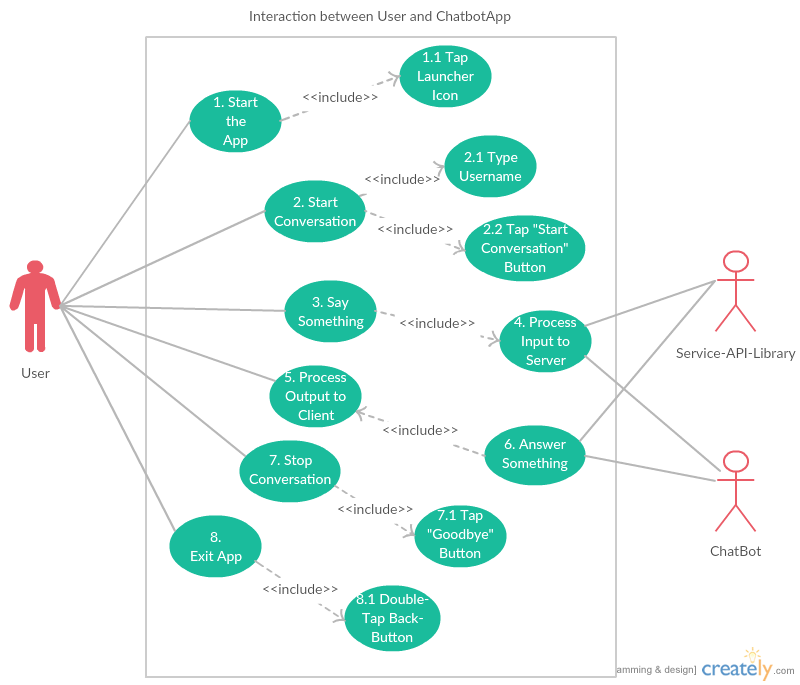
\includegraphics[height=0.5\linewidth]{media/images/android/uc-app.png}}
\end{frame}			
		\begin{frame}
%\frametitle{Gemeinsamkeiten und Unterschiede}
%\framesubtitle{Systemsicherheit}

\begin{block}{}
	example
\end{block}
\begin{block}{}
	more example
\end{block}
\begin{block}{}
	even more example
\end{block}
\end{frame}
	\subsection{Service API}
		\begin{frame}

\begin{block}{}
	Ziel: Vereinfachung der Nutzung des Backend-Servies
\end{block}
\begin{block}{}
	Zentrale Entwicklung der API Bibliothek
\end{block}
\begin{block}{}
	Einheitliche Bibliothek nutzbar in verschiedenen Applikationen (App, Desktop, etc)
\end{block}

\end{frame}
		\begin{frame}

\begin{block}{}
	Maven zur Organisation des Buildvorgangs und der Abhängigkeiten
\end{block}
\begin{block}{}
	Mashape Unirest als Rest-Client
\end{block}
\begin{block}{}
	Je Service Methode eine Methode in der API
\end{block}
\begin{block}{}
	Komplett asynchron nutzbar
\end{block}

\end{frame}
	\subsection{Backend}
		\section{Überarbeitung der Server-Architektur}
	Im Rahmen der Projektarbeit soll die serverseitige Architektur überarbeitet
	und mit der Nutzung von modernen Tools und Frameworks ausgestattet werden.
	Diese Optimierungen werden in den folgenden Unterkapiteln beschrieben.
	
	\subsection{Datenbank}
		Eine Anforderung an das Projekt war es, dass die bisherige Nutzung einer
		Oracle Datenbank abgelöst wird durch eine frei verfügbare Datenbank. Das Team
		entschied sich für das freie relationale Datenbankmanagementsystem MySQL in
		der aktuellsten produktiven Version 5.6.26 zum Zeitpunkt dieser Arbeit.
		Dies bringt den großen Vorteil mit sich, eine weitverbreitete quelloffene, statt
		einer proprietären Datenbank Software zu nutzen.
		
	\subsection{Das Spring Framework}
		Eine weitere Anforderung stellt die Nutzung moderner Frameworks und
		Technologien dar. Um einerseits einen guten Programmierstil sicher stellen zu
		können und andererseits die Kollaboration zu verbessern, sowie zukünftigen
		Projektteams den Einstieg maßgeblich zu erleichtern.
		Spring ermöglicht es durch so genannte Annotationen die Persistierung von
		Objekten unter Zuhilfenahme von Hibernate mit Object-Relational-Mapping zu
		vereinfachen. Zusätzlich wird das Testen mit Unittests durch JUnit
		simplifiziert und die Instanziierung von Objekten zur Laufzeit im
		Singleton-Pattern durchgeführt. Das Speichern und Lesen von Objekten kann
		unter Spring beispielsweise durch Interfaces mit der @Respository Annotation
		übernommen werden. So ist es möglich ohne eine SQL Anweisung selbst zu
		schreiben, Datenbankzugriffe zu realisieren und mit Objekten zu arbeiten.
		Dies erleichtert das Erstellen der Daten-Zugriffsschicht enorm. Diese
		Fähigkeit wird durch das Beerben des Interfaces CrudRepository, oder eines
		davon erbenden Interfaces erworben. Das Beerben eines dieser Interfaces
		verpflichtet zu den grundlegenden Datenbankoperationen Create, Read, Update
		und Delete eines spezifischen Objekttyps. Somit können POJOs in der
		Datenbank direkt abgespeichert werden. Diese werden in Form von separaten
		Model-Klassen angelegt, mit der @Entity Annotation versehen und sind somit
		als Datenbank-Entität gekennzeichnet. Weiterhin kann der Tabellenname, sowie
		einzelne Spaltennamen angegeben werden und Kardinalitäten zu anderen POJOs
		festgelegt werden, z.B. hat eine Kategorie mehrere Themengebiete.\\
		Die Spring Hierarchie ist ein wesentlicher Bestandteil der neu designten
		Server-Architektur und soll hier deshalb zusätzlich Einzug erhalten. Wie
		bereits erwähnt können einzelne Interfaces mit der @Repository Annotation für
		ORM genutzt werden. Diese Datenbankschicht der Hierarchie ist die unterste
		der drei und wird von der darüber befindlichen Service-Ebene genutzt. Hier
		werden Klassen mit der @Service Annotation zum Service ermächtigt, was dem
		Spring Kontext mitteilt, dass diese Services zur Laufzeit als Singleton
		Instanziiert werden. Services nutzen also die darunter liegenden Repositories
		für den Datenbankzugriff und verarbeiten die Daten weiter, bzw. führen andere
		gewünschte Operationen aus. Services stellen also Logikschicht dar. Diese
		Logikschicht wird von der API, den sogenannten Controllern genutzt, um
		Anfragen, sogenannte Web-Requests in Form eines GET oder POST, weiter
		bearbeiten zu können. Ein Controller hält die @Autowired Annotierten Services
		und dieser wiederum die Repositories und diese Objekte werden zur Laufzeit
		Instanziiert.
\section{Aussicht}
	\begin{frame}
\begin{block}{}
	Implementieren weiterer Extensions
\end{block}
\begin{block}{}
	Absichern der Kommunikation per TLS
\end{block}
\begin{block}{}
	Realisieren einer Pädagogenschnittstelle
\end{block}
\begin{block}{}
	todo
\end{block}
\end{frame}

\end{document}
